\section{Изучение свойств управляемого объекта}
На этапе аналитического конструирования системы управления  изучение свойств управляемого объекта выполняется по его математической модели. Модели процессов в объекте могут быть представлены в различных видах. Рассмотрим некоторые из них на примере одномерного объекта, процессы в котором описываются нелинейным дифференциальным уравнением третьего порядка.

\subsection{Исходные данные}
 Разработать управляющее устройство, обеспечивающее 
качественные показатели системы, указанные в 
табл.\ref{tab:
init_cond
}
.
Помимо этого характер переходного процесса должен быть 
апериодическим
, а время переходного процесса должно быть минимально возможным.

\begin{table}[!h] \centering
    \caption{
    Условия задания
    } \label{tab:
    init_cond
    }
    \begin{tabular}{|c|c|c|c|c|c|c|c|}
        \hline
        $T$ & $K$ & $h$ & $d$ & $\sigma_{max},\%$ & $\epsilon_{max},\%$ & $L_{m\,max},db$ & $\gamma,^{\circ}$ \\ \hline
         $9$ & $3$ & $6$ & $0.6$ & $10$ & $1$ & $20$ & $60$ \\ \hline
    \end{tabular}
\end{table}
$\sigma_{max},\%$ --- показатель перерегулирования;

$\epsilon_{max},\%$ --- максимально допустимое отклонение выходной координаты в установившемся режиме;

$L_{m\,max},db$ --- запас устойчивости в "малом" по амплитуде;

$\gamma,^{\circ}$ --- запас устойчивости в "малом" по фазе.
\subsection{Модель объекта в виде СС}
Модель объекта в виде СС представлена на рис. \ref{fig:sim_object}.
\begin{figure}[!h]\centering
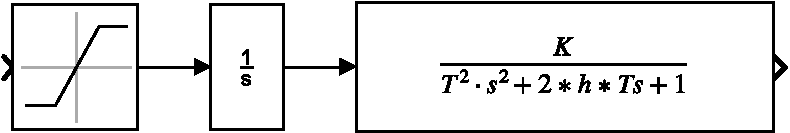
\includegraphics[width=\linewidth]{images/sim_object}
\caption{Структурная схема управляемого объекта.}\label{fig:sim_object}
\end{figure}
\subsection{Модель объекта в виде дифференциального уравнения }
Уравнение \eqref{eq:dif_object_sym} записано в символьном виде с параметрами, а \eqref{eq:dif_object} записано с подстановкой значений параметров.
\begin{equation}\label{eq:dif_object_sym}    \left\{    \begin{aligned}p\,\left(T^2\,p^2+2\,h\,T\,p+1\right)\,x&=K\,u&&, \text{ если}|u|\le d\\p\,\left(T^2\,p^2+2\,h\,T\,p+1\right)\,x&=K\,d\,\mathrm{sign}\left(u\right)&&, \text{ если}|u|>d    \end{aligned}    \right.\end{equation}
\begin{equation}\label{eq:dif_object}    \left\{    \begin{aligned}p\,\left(81\,p^2+108\,p+1\right)\,x&=3u&&, \text{ если}|u|\le 0.6\\p\,\left(81\,p^2+108\,p+1\right)\,x&=1.8\mathrm{sign}\left(u\right)&&, \text{ если}|u|> 0.6    \end{aligned}    \right.\end{equation}
\subsection{Модель управляемого объекта в пространстве состояний }
Уравнение \eqref{eq:ss_object} записано с подстановкой значений параметров.
\begin{equation}\label{eq:ss_object}    \left\{    \begin{aligned}x_1&=x , \\ \cfrac{d\,x_1}{d\,t}&=x_2 ,\\ \cfrac{d\,x_2}{d\,t}&=x_3,\\\cfrac{d\,x_3}{d\,t}&=    \left\{    \begin{aligned}-&
0.0123
\,x_2-
1.3333
\,x_3+
0.0370
\,u&&, \text{ если}|u|\le 
0.6
\\-&
0.0123
\,x_2-
1.3333
\,x_3+
0.0222
\,\mathrm{sign}\left(u\right)&&, \text{ если}|u|> 
0.6
    \end{aligned}    \right.    \end{aligned}    \right.\end{equation}
\subsection{Исследование системы подачей на вход типового воздействия}
Найдём переходную характеристику $h(t)$.
На вход подаём ЕСФ $u=1(t)$
Модель системы в simulink представлена на рис. \ref{fig:sim_object_analysis}.
Переходная характеристика объекта по выходной координате и её скорости представлена на рис. \ref{fig:object_analysis}.
Здесь $x,y,x_1,y_1$ --- это соответственно выходная координата системы с нелинейным элементом, скорость изменения выходной координаты системы с нелинейным элементом, выходная координата системы без нелинейного элемента, скорость изменения выходной координаты без нелинейного элемента.
\begin{figure}[!h]\centering
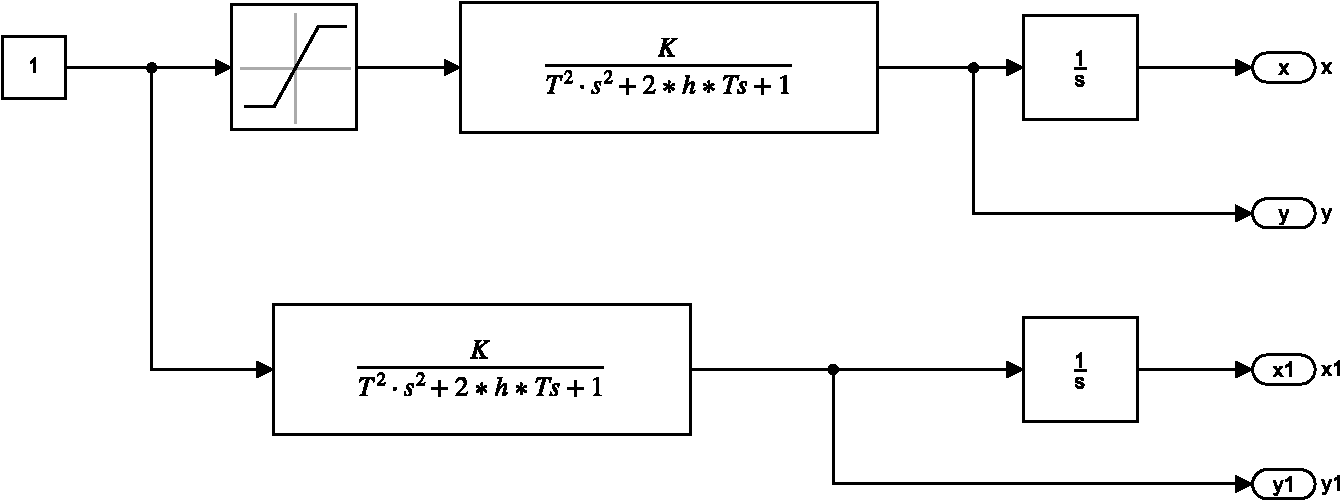
\includegraphics[width=\linewidth]{images/sim_object_analysis}
\caption{Модель системы в simulink.}\label{fig:sim_object_analysis}
\end{figure}
\begin{figure}[!h]\centering
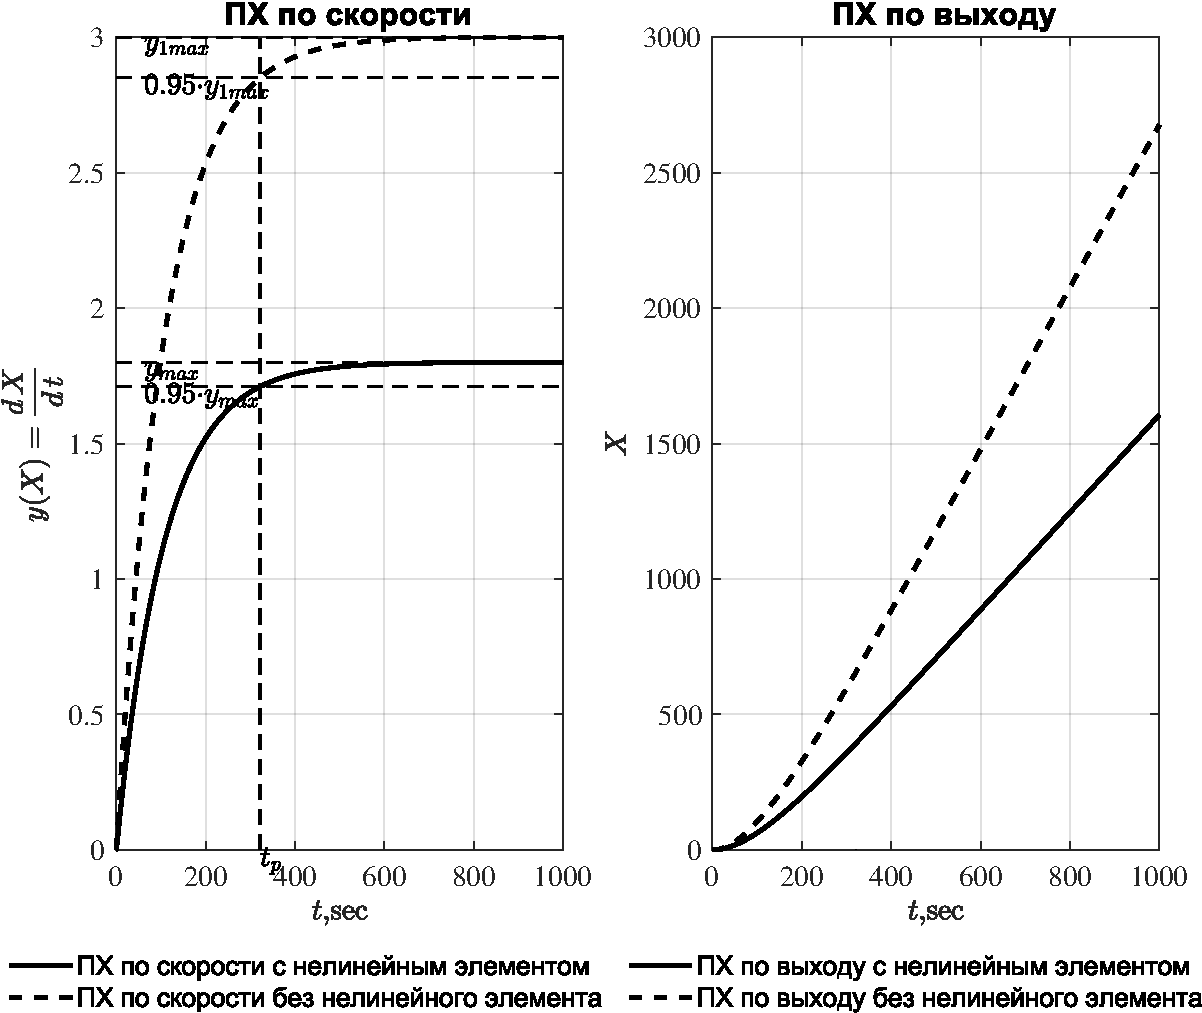
\includegraphics[width=\linewidth]{images/object_analysis}
\caption{Переходная характеристика объекта по выходной координате и её скорости.}\label{fig:object_analysis}
\end{figure}

При подаче на вход ступенчатого воздействия выходная координата теоретически неограниченно возрастает, скорость её изменения также растет, но её рост постепенно замедляется и приходит к установившемуся значению за $t_p=
322$
секунд. Установившиеся значения скорости указаны в таблице \ref{tab:steady_speed}.

\begin{table}[!h] \centering
    \caption{Установившиеся значения скорости} \label{tab:steady_speed}
    \begin{tabular}{|c|c|}
        \hline
        С НЭ & Без НЭ \\ \hline
        1.8 & 3 \\ \hline
    \end{tabular}
\end{table}
Заметим также, что эти значения соостветствуют коэффициентам усиления системы с НЭ и без НЭ.

При этом у системы с нелинейным элементом мгновенные значения выхода и скорости меньше , чем у системы без нелинейного элемента, потому что НЭ в объектк управления типа <<насыщения>> ограничивает максимальное значение сигнала, подаваемого на следующие за ним линейные звенья.

